\documentclass[9pt,twocolumn,twoside]{pnas-new}
% Use the lineno option to display guide line numbers if required

\templatetype{pnasresearcharticle} % Choose template 
% {pnasresearcharticle} = Template for a two-column research article
% {pnasmathematics} %= Template for a one-column mathematics article
% {pnasinvited} %= Template for a PNAS invited submission

\title{Context-dependent selection as the keystone in the somatic evolution of cancer}

% Use letters for affiliations, numbers to show equal authorship (if applicable) and to indicate the corresponding author
\author[1,2]{Vibishan B.}
\author[1,2,*]{Milind G. Watve} 
%\author[a]{Author Three}

\affil[1]{Department of Biology, Indian Institute of Science Education and Research (IISER), Pune}
%\affil[b]{Affiliation Two}
%\affil[c]{Affiliation Three}

% Please give the surname of the lead author for the running footer
\leadauthor{} 

% Please add here a significance statement to explain the relevance of your work
\significancestatement{As opposed to the contemporary mutation-cenrtic perspective, selective forces, at the level of both the organism and the population, play important roles in cancer progression. We construct models of non-selective and selective forces, and compare their predictions of population-level cancer incidence to available epidemiological data from US populations. We find that incorporating selection, particularly selection that varies across organisms in a heterogenous population, is necessary to explain observed trends in cancer incidence. We posit that this heterogenous selection stems from factors that affect the tumour micro-environment that determine the competitive advantage to cancer-causing somatic mutations.}

% Please include corresponding author, author contribution and author declaration information
%\authorcontributions{Both authors conceptualised the work. V.B. wrote the code, and both authors analysed the data and wrote the manuscript.}
\authordeclaration{The authors declare that there are no conflicts of interest}
\equalauthors{\textsuperscript{2}B.V. and M.G.W. contributed equally to this work.}
\correspondingauthor{\textsuperscript{*}To whom correspondence should be addressed. E-mail: milind@iiserpune.ac.in}

% Keywords are not mandatory, but authors are strongly encouraged to provide them. If provided, please include two to five keywords, separated by the pipe symbol, e.g:
\keywords{Somatic evolution $|$ Mutation accumulation $|$ Epidemiology $|$ Cancer etiology $|$} 

\begin{abstract}
Somatic evolution of cancer involves a series of mutations and accompanying genomic, epigenomic and physiological changes in one or more clones of cells. Whether the mutations accumulate by chance alone (``bad luck'' hypothesis) or necessarily involve selection on intermediate mutants leading to clonal expansion is unclear. An implicit assumption in clonal expansion is that any mutation leading to partial loss of regulation of cell proliferation will give a selective advantage to the mutant. However, a number of experiments show that an intermediate pre-cancer mutant has only a conditional selective advantage; given that tissue microenvironmental conditions are differ across individual organisms, the selective advantage to a mutant will be widely distributed over the population of organisms. We comparatively evaluate the three models, namely ``bad luck'', context-independent selection and context-dependent selection with respect to their ability to predict patterns in total incidence, age-specific incidence, and their ability to explain Peto’s and related paradoxes. Results show that the number of stem cells and mutation rates are unlikely to be rate limiting in human cancers, and that context dependence is necessary and sufficient to explain all the observed epidemiological patterns. This implies that the susceptibility to cancer can be substantially different across individuals, and cancer is not sheer bad luck. A wide range of physiological, genetic and behavioural factors influence the tissue micro-environment, and could therefore be the source of this context dependence in somatic evolution of cancer. The identification and targeting of these micro-environmental factors that influence the dynamics of selection offer new possibilities for cancer prevention.
\end{abstract}

\dates{This manuscript was compiled on \today}
\doi{\url{www.pnas.org/cgi/doi/10.1073/pnas.XXXXXXXXXX}}

\begin{document}

\maketitle
\thispagestyle{firststyle}
\ifthenelse{\boolean{shortarticle}}{\ifthenelse{\boolean{singlecolumn}}{\abscontentformatted}{\abscontent}}{}

% If your first paragraph (i.e. with the \dropcap) contains a list environment (quote, quotation, theorem, definition, enumerate, itemize...), the line after the list may have some extra indentation. If this is the case, add \parshape=0 to the end of the list environment.
\dropcap{O}ver the past 60 years or so, ideas in the field of cancer epidemiology have evolved significantly, with the first models starting from the Armitage-Doll multi-stage models \cite{ARMITAGE1954}, which predicted a power law relationship of cancer risk with age. The connection between the multiple stages and sequential genetic mutation events was established definitively for retinoblastoma with the two-hit hypothesis \cite{Knudson1971}. This finding has since directed a lot of attention to mutational processes and genetic instability within cells as fundamental forces in cancer, and their signatures in population-level datasets; Tomasetti et al. have made the argument for cancer risk being largely determined by random mutations \cite{Tomasetti78, Tomasetti2017}, and others have studied the impact of selectively-neutral or deleterious passenger mutations on the expansion and progression of advantageous mutant clones \cite{McFarland2013}, mutation accumulation rates across tissue types \cite{Blokzijl2016}, or dependencies between mutations \cite{Mina2017}. On the other hand, an old debate in the theory of evolution is how the simple process of random mutations and natural selection can lead to compled structures such as the eye, that need coordinated action of several genes. This is often perceived as a monkey-on-a-typewriter paradox \cite{Dawkins1996}-how likely is it that a monkey sitting at a typewriter and hitting keys at random would end up typing a meaningful sentence? The problem of cancer is qualitatively similar to this, but quantitatively even more difficult, as no single mutation is known to make a cell cancerous. All cancers are necessarily a combination of different types of genomic changes including point mutations, aneuploidy, and other chromosomal aberrations. The cancer phenotype has a large number of distinguishing characeters, encapsulated by the notion of the ``hallmarks'' of cancer \cite{Hanahan2000, Schafer2008, Hanahan2011}, and the wide range of characterisitics that these hallmarks include make it astonishing that so many alterations in cell properties come together in cancers purely out of chance, especially since most cancers must evolve independently in each individual organism.

Selection was clearly required to explain the complex cancer phenotype, clonal expansion provided the first such instance of a selective evolutionary process. Every component mutation on the way to a cancerous phenotype causes the mutant clone to expand, and as the mutant population increases, the probability of a second component mutation increases proportionately \cite{Nowell1976}. Implicit in this theory is the assumption that every component mutation has a selective advantage over the normal cell. Since most changes involved in carcinogenesis relate to evading growth regulatory mechanisms, it is considered logical that any mutation that allows for such evasion will have a natural selective advantage. However, evidence has been accumulating over the past few years that the fitness advantage of a mutant is largely dependent on the tissue micro-environment \cite{Hanahan2012, Pietras2010}. Studies in mice \cite{Cao2010} and humans \cite{Rundqvist2013} have demonstrated the effect of contingent factors, such as behavioural profiles and lifestyle parameters, on cancer progression. Such findings provide clear indications that the selective forces which determine mutant clone fitness can vary considerably across individual organisms, leading to \textit{context-dependent clonal expansion} of potentially oncogenic mutants. This aspect of cancer progression has seen some modeling effort in the past few years \cite{Nagy2007, Caulin2011, Hochberg2017}, but a part of the legacy from Armitage-Doll has been partly lost. The first models in cancer etiology involved comparison of model predictions with epidemiologically-observed trends in incidence. This framework allowed for comparison of competing theories of carcinogenesis based on how closely they agreed with epidemiological data, and we construct a similar framework here, to evaluate competing causal factors in cancer etiology based on comparisons with data from the US population \cite{AmericanCancerSociety2016}.

Across biological levels, we identify at least three processes that seem to play a major role in cancer progression and etiology, two of which, explicitly include selection at different levels: (1) random mutagenesis, or the ``bad luck'' hypothesis, (2) expansion of mutant clones within organisms, and (3) context-dependent selection acting across organisms. Since well-curated data is available for human cancer incidence patterns, we develop models of these three processes, and compare their predictions with the epidemiological picture of cancer in the human population. We briefly summarize the essential epidemiological features that must be part of any comparative modeling framework:

\begin{enumerate}
	\item Total and age-specific incidence: Across cancer types, total population-level incidence lies around 20 to 30\%, while age-specific and cumulative incidence patterns show more variations \cite{AmericanCancerSociety2016}. Interestingly, recent analyses have shown for several cancer types that the age-specific incidence rates decline late in life, in contrast with general model predictions of a power law increase in incidence with age \cite{Harding2012}. The late-life decline causes the cumulative incidence to saturate with age at a small percentage of the population size, which is an important detail. No matter the lifespan, the proportion of cancer in the population can never reach 100\%, which represents a finite limit that is not determined by time.
	\item Incidence vs cell number: As mentioned earlier, the relationship between cancer risk and cell number (as the lifetime number of cell divisions, \textit{lscd}) has been kept in the spotlight by recent work by Tomasetti et al. \cite{Tomasetti78, Tomasetti2017}. On the whole, the linearity of the relationship between \textit{lscd} and cancer risk is still under debate, although an explanation of this non-linearity remains incomplete. We think that the relationship is non-linear, and possibly saturating, as is clear from an examination of the slopes of the cancer risk-\textit{lscd} association. Linear or not, there are still real-life data for the relationship with which model predictions may be compared; as we show later, the veracity of the linearity claim is not directly relevant to the conclusions we draw from our models.
	\item Incidence vs mutation rate: Empirical data on this relationship are less common, as mutation rates are difficult to measure reliably, although some efforts have been made \cite{Hao2016}. However, a general notion exists that higher mutation rates increases cancer risk, and this remains to tested rigorously, barring theoretical work dealing with the effect of mutagens on patterns in incidence data \cite{Frank2007}.
	\item Non-mutagenic carcinogens: There are several agents, including hormones and growth factors, that increase cancer risk without affecting the basal mutation rate [citations]. The activity of these agents, and their signature in epidemiological patterns, are both important in building a complete framework of explaining cancer etiology.
	\item Peto's paradox, and similar observations: This relates to the incidence-cell number relationship, as cancer risk is seen not to scale with body size or cell number across species \cite{Nagy2007}, with does correlate with the latter within a species \cite{Noble2015}. A wide range of explanations have been offered for this observation \cite{Tollis2017b}, but a comprehensive explanation has been elusive. Nevertheless, it remains an key feature of cancer etiology with regard to the modeling effort.
	%\item Mutational meltdown: While well-known in other study systems, the effects of deleterious mutations were recognized relatively recently in cancer literature.
\end{enumerate}


\section*{The ``bad luck'' model}

This hypothesis assumes that the required set of driver mutations accumulate in a cell by chance alone. This may happen over a period of time, or in a single large-scale event, like chromothripsis \cite{Stephens2011}. Regardless of whether mutations accumulate sequentially or otherwise, the ``bad luck'' model does not assume selection of any kind on mutations over the course of somatic evolution.

Consider an organism with a population of $n$ stem cells, each with a mutation rate per cellular generation per locus, $p$. The probability that at least one cell acquires one mutation at a given point of time can be given as $1-(1-p)^{n}$. If $k$ such mutations are requried for cancer onset, the probability of cancer according to the bad luck model can be given as below, based on an algebraic formulation \cite{Calabrese2010}:

\begin{equation}
	\label{E1}
	p_{can} = 1-(1-p^{k})^{n}
\end{equation}

Given the probability of cancer per unit time, $p_{can}$ from equation \ref{E1}, the cumulative incidence of cancer for age, $A$, can be expressed as below:
\begin{equation}
	\label{E2}
	p_{A} = 1-(1-p_{can})^{A}
\end{equation}

From equation \ref{E1}, it is clear that the probability of cancer has a threshold relationship with both $n$ and $p$, such that incidence rises from near zero to 100\% over a small range of $p$ and $n$, as shown in Figure \ref{fig1}. Within this narrow range, total incidence as reflected by the cumulative probability, $p_{can}$, occasionally lies in the realistic range of about 30\%, but these are the exceptions.

\begin{figure*}[tbhp]
	\centering
	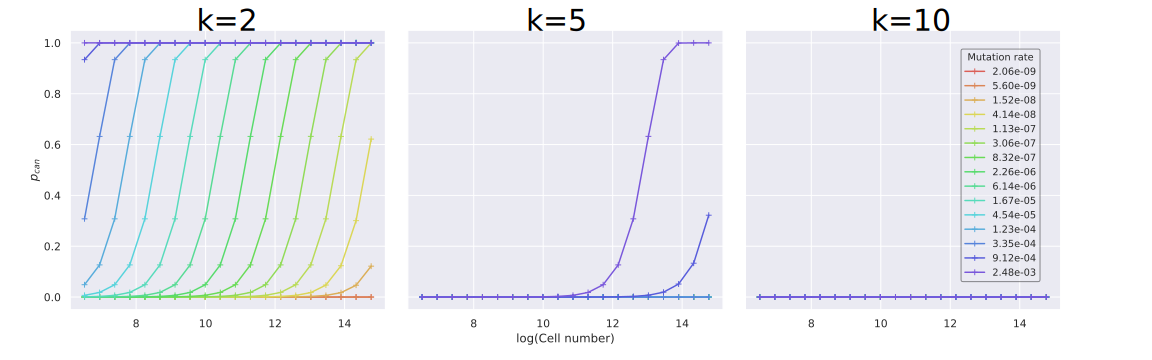
\includegraphics[width=.8\linewidth]{fig1.png}
	\caption{Cancer probability, $p_{can}$ vs mutation rate and cell number for the ``bad luck'' model; $p_{can}$ remains near zero in part of the parameter range, and rises to one over a narrow region of the corresponding parameter. This proability is cumulative and therefore reflects total incidence in the population. For the ``bad luck'' model, the total incidence is rarely in the observed range of around 30\%. The number of oncogenic mutations required for cancer onset ($k$) does not affect the existence of a threshold with $n$ and $p$, but does affect where the threshold occurs in the parameter space; for $k=10$, the threshold does not occur within the tested range of $n$ and $p$. The legend shows values of $p$ for each curve.}
	\label{fig1}
\end{figure*}

From equation \ref{E2}, the relationship of $p_{can}$ with age is a monotonically increasing function with a maximum at one. Figure \ref{fig2} shows this relationship across the entire parameter range of $n$ and $p$, for which this prediction holds. Cancer probability increases monotonically with age, and only saturates at 100\% incidence, which stands in stark contrast to the observed late-life decline in age-specific rates.

\begin{figure}[tbhp]
	\centering
	\includegraphics[width=.8\linewidth]{fig2.png}
	\caption{Cancer probability vs age, as given by equation \ref{E2}, (A and B) over the range of $n$, and (C and D) over the range of $p$; inset legends give the corresponding values. Cancer probability increases monotonically with age, saturating only at one in most cases. Where the probability does approach realistic values of total incidence, it still does not reflect the late-life decline in incidence rates observed epidemiologically. As in Figure \ref{fig1}, the number of oncogenic mutations required for cancer onset does not change the nature of the incidence-age relationship. For A and C, $k=2$, and for B and D, $k=5$.}
	\label{fig2}
\end{figure}

For the sake of simplicity, we have ignored the cost of lethal and/or passenger mutations, and assume that the mutations occur together at any given point of time; although the model predictions change marginally, we see that this assumption does not affect the general inferences we draw. Taken together, this formulation of the ``bad luck'' model predicts a sharp threshold relationship of cancer probability with both $n$ and $p$, and a monotonically increasing relationship with age, both of which can be falsified based on a simple comparison with published epidemiological data.
%We also used values of $n$ and $p$ for about 15 cancer types, along with the corresponding lifetime incidence of cancer from published literature \cite{Tomasetti78, Hao2016}, to carry out a chi-square test to compare the predictions of the ``bad luck'' model with the SEER incidence. A quick calculation is sufficient to show that the former predicts 100\% incidence for all tested cancer types, which is clearly unrealistic.

While there are ways of incorporating additional complexities within the formulation presented here, we choose to explore the effects of clonal expansion and context-dependent selection through a simulation-based framework. As we show below, it allows for easier exploration of the parameters under study, and creates a logical progression in terms of biological scale; the ``bad luck'' model deals with cell-level properties, clonal expansion is a tissue- or organ-level phenomenon, while context-dependent selection occurs between organisms at the level of the population.

\section*{Models with selection on mutants}
We use a linear process to model the sequential accumulation of mutations in a population of stem cells. We begin by considering the development of a generalized tissue compartment in each organism starting from one stem cell, with mutation rate per cell generation per locus, $p$, growing logistically to a carrying capacity, $n$, following the discrete logistic equation below:
\begin{equation}
	m_{i, t} = m_{i, t-1} + m_{i, t-1}*g_{i}*(\dfrac{n-\sum_{i=0}^{k} m_{i, t-1}}{n}) - m_{i, t-1}*d
	\label{E3}	
\end{equation}

Here, $m_{i, t}$ is the size of the $i$th mutant population at time, $t$, with $i=0$ being the non-mutant cell population, $g_{i}$ is the corresponding logistic growth rate, $d$ is the common death rate, and $k$ is the threshold number of oncogenic mutations required for cancer onset. As the organism develops into an adult, net growth in the stem cell compartment saturates, but reaches a dynamic equilibrium between cell death and renewal. The stem cell population can be reduced, either by death of stem cells, or assymetric division to produce differentiated cells. The death rate in equation \ref{E3} is this constant rate of cell removal from the stem cell population. Assuming a common death rate for all cell populations, the replacement of the lost cells by either mutants or non-mutants is a function of their growth rates. We simulate new mutation events stochastically; the probability of at least one cell accumulating a mutation is given by $1-(1-p)^{m_{i, t}}$, and if this probability exceeds a random number between 0 and 1, a new $(i+1)$th cell population is initiated. We assume that each new oncogenic mutation offers a growth advantage over older cell populations, leading to successive cycles of clonal expansion in which the newer population gradually replaces older cells through competitive exclusion. We simulate this linear evolution process until $k$ mutations have been accumulated, which is the assumed threshold for cancer onset. Death of the organism occurs either at cancer onset when the $k$th mutation occurs, or at the end of the natural lifespan of 100 years, whichever happens first. This simulation is repeated independently for 10000 organisms, and the population-level cancer incidence is recorded, along with the age of onset.
	\subsection*{Choice of parameter range}
	In order to standardize the discrete logistic simulation, we assume the time unit to be one day per logistic growth step. Most human organs complete development and maturation wihtin the first 10-20 years of the lifespan, and the final carrying capacity achieved is the adult stem cell number, ranging between $10^{6}$ and $10^{11}$ across different tissues. Given the final population size and the time taken to reach it, a simple calculation based on the logistic equation shows the required growth rate for a non-mutant stem cell to be in the range of $0.00383$-$0.0131$ [details in the supplement]. Starting from the non-mutant growth rate, $g_{0}$, growth rates are assumed to increase linearly for each subsequent mutant population. For all simulations, we assume $g_{0}=0.007$ to obtain cancer incidence within an organism's lifespan. Ranges of $n$ and $p$ are retained as in the ``bad luck'' model.

	\subsection*{The context-independent selection case}
	While the clonal expansion theory introduced the notion of selective advantages to oncogenic mutants, it makes the implicit assumption that identical mutations have the same selective advantage in every organism in which they occur; stated otherwise, individual organisms do not differ in their propensity for mutant clonal expansion. To capture this in the context-independent selection case, we use the same linear progression of growth rates for all organisms in the simulation.

	\subsection*{The context-dependent selection case}
	As argued earlier, it is becoming increasingly clear that the competitive outcomes of identical mutations can depend strongly on the micro-environmental context in which cell competition occurs. In order for selection on mutants to be context-dependent in our model, we randomize the progression of growth rates during mutation accumulation. Each organism begins with the same $g_{0}$, but the progression of growth rates is randomized across individual organisms, such that organisms with large $g$s would progress faster towards cancer onset, while those with small, or negative values of mutant $g$s would never progress to a cancerous state as the mutant gets selected against. This produces variation across organisms for cancer propensity, leading to a more realistic model.
	%While we study a simple case by randomizing $\mu$, in principle, it should be possible to vary $g_{k}$ with respect any non-random context-dependent variable derived from real data sources. But as we show later, our simple case several interesting results by itself.

\subsection*{Predictions from the selection models}
As Figure 1 shows, under the assumption of context-independent selection, the incidence of cancer shows a strong threshold relatioship with age, where cancer is unlikely or rare up to a certain age, and increases rapidly to 100\% with a relatively short span of time. This is indicated by the fact that the age-specific crude incidence falls sharply to zero at some point in the lifespan, when the cumulative incidence also reaches 100\%. As with the ``bad luck'' model, incidence has a threshold relationship wtih both $n$ and $p$, in terms of the age at half-maximum incidence (Figure \ref{fig3}C and G) and the maximum cumulative incidence, $I_{max}$ (Figure \ref{fig3}D and H). Moreover, saturation of incidence occurs only at 100\%, which is identical to the ``bad luck'' model, despite the inherently stochastic implementation of mutation occurrence. Where the incidence of cancer is near the realistic range, for small values of $p$ and $n$, the late-life decrease in incidence is still not reflected in the context-independent selection case. The prediction of 100\% incidence is due to the fact that all organisms in the population share the same growth rate progression for mutants. No other parameter in the model inherently precludes the accumulation of all k oncogenic mutations in some organisms, and the dynamics of accumulation is entirely a function of $p$ and $n$, along with stochastic variation. The context-independent selection model thus predicts that with increasing $p$ and/or $n$, cancer incidence increases, and reaches saturation only at 100\% incidence. Therefore, clonal expansion accounts for some physiologically-relevant phenomena, like competitive growth of mutants, its description of cancer incidence and the effects of model parameters are either unrealistic, or incomplete.

\begin{figure*}[tbhp]
	\centering
	\includegraphics[width=.8\linewidth]{fig3.png}
	\caption{Incidence patterns from the context-independent selection model over the range of (A-D) $n$, and (E-H) $p$. From left to right in each row, the plots are of (A, E) age-specific crude incidence per 100000 vs age, (B, F) cumulative incidence for the simulated population vs age, (C, G) age at which half the maximum incidence is reached vs $log(n)$ or $log(p)$, and (D, H) the maximum cumulative incidence, $I_{max}$ vs $n$ or $p$. Inset legends for the age curves are $log(n)$ and $log(p)$ in the top and bottom row respectively. For A-D, $p=5.603*10^{-9}$, and for C-H, $n=1.785*10^{8}$. Insets for the incidence curves show $log(n)$ and $log(p)$ in the top and bottom rows respectively. Growth rates progress linearly in the general form, $g_{i}=0.007*(i+1)$, where $i=0,...,k$ and $k=5$.}
	\label{fig3}
\end{figure*}

As opposed to the context-independent selection model, the context-dependent model produces a saturating trend in cumulative incidence that begins to saturate at a level much lower than 100\%. As Figure \ref{fig4} shows, the saturation limit for many values of ‘n’ and ‘p’ is quite close to the epidemiological estimate of cancer risk (20-30\%). This is an important feature of the context-dependent model, as it allows the model to generate more realistic patterns in age-specific cancer incidence. The realistic saturation of population incidence can be explained by the fact that propensity for clonal expansion varies across organisms, such that cancer progression occurs very quickly in some organisms, and not at all in others. Of the three models analysed so far, only the context-dependent model captures a trend similar to the late-life decline observed in many cancers in humans as the crude incidence curves in Figure \ref{fig4}A and E show, which suggests alternative explanations for trends in cancer incidence, independent of possible evovled cancer defenses.

\begin{figure*}[tbhp]
	\centering
	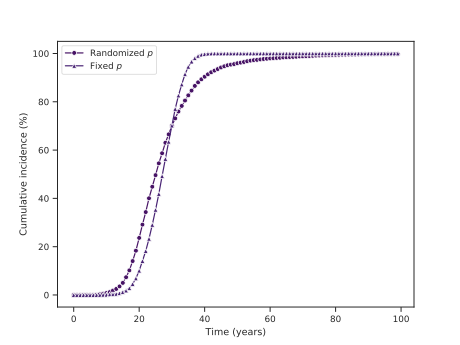
\includegraphics[width=.8\linewidth]{fig4.png}
	\caption{Incidence patterns from the context-dependent selection model over the range of (A-D) $n$, and (E-H) $p$. From left to right in each row, the plots are of (A, E) age-specific crude incidence per 100000 vs age, (B, F) cumulative incidence for the simulated population vs age, (C, G) age at which half the maximum incidence is reached vs $log(n)$ or $log(p)$, and (D, H) the maximum cumulative incidence, $I_{max}$ vs $n$ or $p$. Inset legends for the age curves are $log(n)$ and $log(p)$ in the top and bottom row respectively. For A-D, $p=5.603*10^{-9}$, and for C-H, $n=1.785*10^{8}$. Insets for the incidence curves show $log(n)$ and $log(p)$ in the top and bottom rows respectively. Growth rates progress linearly from $g_{0}=0.007$ to $g_{k}=0.007*\mu$, where $\mu$ is normally-distributed random variable with $\overline{\mu}=0$ and $\sigma=3$, and $k=5$.}
	\label{fig4}
\end{figure*}

\section*{Sensitivity of predictions}
For all the simulations so far, we have assumed $k=5$ under all conditions, randomizing only the other parameters. Real populations, on the other hand, could potentially be a heterogenous mix of $k$ across organisms, which might affect the model predictions. To explore this possibility, we co-randomized $k$ with either $n$ or $p$ while maintaining the same growth rate progression, and looked at the association of $log(n)$ or $log(p)$ with the time taken for cancer onset. The time taken to cance is a useful parameter as it describes temporal mutation accumulation dynamics directly, while allowing for some limited inference regarding total incidence in the population. If time taken to cancer is largely small, population incidence is likely to be large in the given parameter space.
Broadly, we find that cancer incidence is significant only up to maximum $k=10$. Increasing $k$ also reduces total incidence and shifts the observed time to cancer to later in life (Figure \ref{figS1}), as expected based on mutation accumulation. We also find that the magnitude of $k$ could modulate the strength of the association $n$, and to a lesser extent, with $p$. Doing the same for the context-dependent case, we randomized $g$ as explained earlier, along with either $k$ and $n$, or $k$ and $p$. Remarkably, introducing $g$ as a random variable leads to most of the variance in time to cancer being explained by $g$, and to some extent, $n$. Together, this indicates that independent of the kind of selection assumed in the model, $k$ influences the expected effect of $n$, $p$ and $g$ on time to cancer, and that $g$, when randomized, is a stronger predictor than $p$ or $n$ alone.

We have also assumed a normal distribution for the growth rate progression in the simulations so far. Realistic estimates of the distribution of somatic mutant growth rates are currently unknown, but heavy-tailed distributions like the Gumbel distribution have been considered a possibility \cite{Durrett2010}. We have reevaluated the predictions of the context-dependent selection model, for two distributions of $g$, Gumbel and uniform. We find that the shape of the distribution does not affect the nature of the relationships predicted by the model, although some quantitative differences ocur as expected (Figure \ref{figS3}.



\section*{Discussion}
%
\begin{table*}[tbhp]
\centering
\caption{Summary of model predictions vs observed trends}
\begin{tabular}{p{5cm}p{4cm}p{4cm}p{3.5cm}p{7cm}}
\textbf{Epidemiological observation} & ``Bad luck'' & Context-independent selection & Context-dependent selection \\
\midrule
\textbf{Total incidence across cancer types does not exceed 30\%} & Saturation at 100\% only & Saturation at 100\% only & Saturation<100\% possible \\
\textbf{Age-specific incidence decreases in old age for several cancers} & No late-life decline & No late-life decline & Late-life decline predicted \\
\textbf{Incidence vs $n$} & Strong threshold saturating at 100\% & Strong threshold saturating at 100\% & Progressive increase \& saturation<100\% \\
\textbf{Incidence increases progressively with $p$, but not indefinitely} & Strong threshold saturating at 100\% & Strong threshold saturating at 100\% & Progressive increase \& saturation<100\% \\
\textbf{Non-mutagenic carcinogens increase cancer risk, but not the mutation rate} & Incompatible & Incompatible & Explained based on $g$ distribution \\
\textbf{Peto's paradox} & Insufficient & Insufficient & Cancer risk saturates with $n$ \\
\bottomrule
\end{tabular}
%\addtabletext{nomenclature for the TSs refers to the numbered species in the table.}
\end{table*}

%Returning to the epidemiological patterns in the introduction, we now review the predictions of the three models. The ``bad luck'' model predicts a strong threshold of cancer probability with $n$, $p$ and with age. In all three cases, incidence increases in a roughly sigmoid fashion, and saturates only at 100\% incidence. This is also broadly true of the context-independent selection model, which similarly fails to capture the saturation of incidence at around 30\% in real populations, along with the late-life decline in age-specific incidence observed in several cancer types. Along the same lines, the sharp threshold relationships from both of these models of incidence with both $n$ and $p$ stand in clear contrast to real data. As stated earlier, the relationship between incidence and cell number is claimed to be linear by man in the field \cite{Tomasetti78, Tomasetti2017}. While it remains to be conclusively determined if this relationship indeed is linear or non-linear, there is sufficient basis to reject the threshold prediction from the ``bad-luck'' and context-independent selection model. Regardless of whether we assume linearity over a large range of $n$, or general non-linearity, the actual relationship is still a progressively increasing function of incidence with $n$ where the first two models predict a strong threshold effect. While a similarly detailed look is not possible with current data for the relationship of incidence with $p$, there is again sufficient basis to reject a sharp threshold and/or 100\% incidence as predicted by the ``bad luck'' and context-independent models.

%On all these counts, we see that the context-dependent selection offers much more realistic predictions for the relationship of incidence with $n$, $p$ and age. It can produce saturation of incidence at around observed rates in real populations, the observed late-life decline in incidence, and more realistic relationships with $n$ and $p$. It has also indicated interesting effects of the number of oncogenic mutations required for cancer. While it is expected that higher $k$ increases the time taken for cancer onset, the value of $k$ is also seen to modulate how strongly $n$, $p$ and $g$ affect the time to cancer onset, particularly in the moderate to higher range of $k$. This is an important detail that pan-cancer analyses of incidence trends must take note of. For small values of $k$, $n$ does not affect incidence dynamics, but $g$ and $p$ do. The context-dependent model also offers potential explanations for the late-life decline in age-specific incidence. In the model, we see that cancer incidence is determined to a large extent by $g$, suggesting a selection-limited process. Late-life incidence in the model comes from a slow growth rate progression across mutations, and a late-life decline can therefore be described in terms of the distribution of the growth rate progression. In a population where slow growth rate progression for mutants is rare, organisms with active mutagenesis progress to cancer relatively earlier in life, and cancer is rarer later in life. It becomes important therefore, to consider the local or evolutionary factors underlying such a temporal pattern of mutation accumulation. 

On the whole, the better prediction profile of the context-dependent model stems from the distribution of $g$ in the population, and this has interesting implications for the kind of causal factors that are important in explaining cancer etiology. One of these implications concern the mutation-centric thinking that characterizes a good portion of current opinion in cancer biology. For instance, several growth factors and hormones are known to increase cancer risk, not the least of which is insulin, without increasing the basal mutation rate or the cell number. The action of such ``non-mutagenic carcinogens'' is not compatible with a mutation-centric approach to carcinogenesis. We propose instead that parameters like $g$, which reflect context-dependent selection on mutants, offer better explanative scope.
Similarly, late-life incidence in the model comes from a slow growth rate progression across mutations, and a late-life decline can therefore be described in terms of the distribution of the growth rate progression. In a population where slow growth rate progression for mutants is rare, organisms with active mutagenesis progress to cancer relatively earlier in life, and cancer is rarer later in life. It becomes important therefore, to consider the local or evolutionary factors underlying such a temporal pattern of mutation accumulation.
This line of thinking can also be extended to address Peto's paradox. It is not a new argument that Peto's paradox can be explained by invoking selection \cite{Caulin2011,Noble2015,Tollis2017b}. The results from our model in fact reinforce the notion that the processes underlying Peto's paradox, and other related observations, are largely selection-limited, which explains why cancer risk does not increase in proportion with cell number and/or body size. Moreover, our analysis introduces the additional dimension of population-level variation in cancer propensity as part of the explanation of Peto's paradox, and accounting for this variation that lies on top of evolved cancer defences leads to a more nuanced view of the paradox. 
This selection is imposed by the micro-environment in the tumour or pre-cancerous niche, and includes all the factors that determine the selective advantage of oncogenic or pre-cancerous mutant. As mentioned earlier, empirical evidence of such context dependence has been accumulating on multiple fronts. Breast cancer literature is particularly rich in this regard; levels of estrogen and progesterone affect production of growth factors and ECM components by cells \cite{Haslam2001,Woodward2000,DICKSON1987}, and important observations have also been made suggesting synergistic action between hormonal and cytokine-based regulation of cell growth \cite{Freund2003}. The substantial scope of these interactions has been comprehensively reviewed, both for breast cancer particularly \cite{Hansen2000}, and more generally across cancer types \cite{Pietras2010,Hanahan2012,Cabarcas2011a}. For instance, the prohibitive effect of estradiol in ER-negative tumours \cite{Garcia1992} points to the possibility that estradiol reduces the selective advantage of an ER-negative phenotype. More recently, experiments have been reported in which behaviourally-enriched environments or physical exercise seemed to show cancer-suppressive effects \cite{Cao2010,Rundqvist2013} that correlate with secretion of particular growth factors. Independently, the growth factor composition of culture media is also found to markedly alter selective outcomes of mutant phenotypes in cell competition \textit{in vitro} \cite{Archetti2015}, and growth characteristics of pre-cancerous cell lines across cancer stages \cite{Chan2014}. Taken together, these observations offer potential explanations for context-dependent selection on oncogenic mutations, and suggest interesting avenues of transalational importance for cancer prevention and therapy.

A composite view of cancer etiology requires not only the incorporation of these, and other complexities in models, but also the comparative testing framework that continues to be rare in cancer literature, barring a few efforts \cite{Frank2007}. The value of such a framework is immense, as it allows for falsification of factors that make predictions contrary to observed data; this falsification is frequently more robust and informative than an indirect confirmation of potential causal factors. With our analysis, we hope to bring this framework back into the mainstream at a time when the availaibility of large-scale data spanning levels of biological organization is better than ever before, from the population to the various cellular ``-omes''. A comparative framework could prove more powerful now, in the context of robust data and computational techniques, and should therefore become a major focus for the cancer modeling effort.
%\subsection*{Author Affiliations}

%Include department, institution, and complete address, with the ZIP/postal code, for each author. Use lower case letters to match authors with institutions, as shown in the example. Authors with an ORCID ID may supply this information at submission.

%\subsection*{Submitting Manuscripts}

%All authors must submit their articles at \href{http://www.pnascentral.org/cgi-bin/main.plex}{PNAScentral}. If you are using Overleaf to write your article, you can use the ``Submit to PNAS'' option in the top bar of the editor window. 

%\subsection*{Format}

%Many authors find it useful to organize their manuscripts with the following order of sections;  Title, Author Affiliation, Keywords, Abstract, Significance Statement, Results, Discussion, Materials and methods, Acknowledgments, and References. Other orders and headings are permitted.

%\subsection*{Manuscript Length}

%PNAS generally uses a two-column format averaging 67 characters, including spaces, per line. The maximum length of a Direct Submission research article is six pages and a Direct Submission Plus research article is ten pages including all text, spaces, and the number of characters displaced by figures, tables, and equations.  When submitting tables, figures, and/or equations in addition to text, keep the text for your manuscript under 39,000 characters (including spaces) for Direct Submissions and 72,000 characters (including spaces) for Direct Submission Plus.

%\subsection*{References}

%References should be cited in numerical order as they appear in text; this will be done automatically via bibtex, e.g.. All references should be included in the main manuscript file.  

%\subsection*{Data Archival}

%PNAS must be able to archive the data essential to a published article. Where such archiving is not possible, deposition of data in public databases, such as GenBank, ArrayExpress, Protein Data Bank, Unidata, and others outlined in the Information for Authors, is acceptable.

%\subsection*{Language-Editing Services}
%Prior to submission, authors who believe their manuscripts would benefit from professional editing are encouraged to use a language-editing service (see list at www.pnas.org/site/authors/language-editing.xhtml). PNAS does not take responsibility for or endorse these services, and their use has no bearing on acceptance of a manuscript for publication.


%\begin{SCfigure*}[\sidecaptionrelwidth][t]
%\centering
%\includegraphics[width=11.4cm,height=11.4cm]{frog}
%\caption{This caption would be placed at the side of the figure, rather than below it.}\label{fig:side}
%\end{SCfigure*}

%\subsection*{Digital Figures}

%Only TIFF, EPS, and high-resolution PDF for Mac or PC are allowed for figures that will appear in the main text, and images must be final size. Authors may submit U3D or PRC files for 3D images; these must be accompanied by 2D representations in TIFF, EPS, or high-resolution PDF format.  Color images must be in RGB (red, green, blue) mode. Include the font files for any text. 

%Figures and Tables should be labelled and referenced in the standard way using the \verb|\label{}| and \verb|\ref{}| commands.

%Figure \ref{fig:frog} shows an example of how to insert a column-wide figure. To insert a figure wider than one column, please use the \verb|\begin{figure*}...\end{figure*}| environment. Figures wider than one column should be sized to 11.4 cm or 17.8 cm wide. Use \verb|\begin{SCfigure*}...\end{SCfigure*}| for a wide figure with side captions.

%\subsection*{Tables}
%In addition to including your tables within this manuscript file, PNAS requires that each table be uploaded to the submission separately as a “Table” file.  Please ensure that each table .tex file contains a preamble, the \verb|\begin{document}| command, and the \verb|\end{document}| command. This is necessary so that the submission system can convert each file to PDF.

%\subsection*{Single column equations}

%Authors may use 1- or 2-column equations in their article, according to their preference.

%To allow an equation to span both columns, use the \verb|\begin{figure*}...\end{figure*}| environment mentioned above for figures.

%Note that the use of the \verb|widetext| environment for equations is not recommended, and should not be used. 

%\begin{figure*}[bt!]
%\begin{align*}
%(x+y)^3&=(x+y)(x+y)^2\\
%      &=(x+y)(x^2+2xy+y^2) \numberthis \label{eqn:example} \\
%      &=x^3+3x^2y+3xy^3+x^3. 
%\end{align*}
%\end{figure*}


%\begin{table}%[tbhp]
%\centering
%\caption{Comparison of the fitted potential energy surfaces and ab initio benchmark electronic energy calculations}
%\begin{tabular}{lrrr}
%Species & CBS & CV & G3 \\
%\midrule
%1. Acetaldehyde & 0.0 & 0.0 & 0.0 \\
%2. Vinyl alcohol & 9.1 & 9.6 & 13.5 \\
%3. Hydroxyethylidene & 50.8 & 51.2 & 54.0\\
%\bottomrule
%\end{tabular}

%\addtabletext{nomenclature for the TSs refers to the numbered species in the table.}
%\end{table}
%


%\subsubsection*{SI Datasets} 

%Supply Excel (.xls), RTF, or PDF files. This file type will be published in raw format and will not be edited or composed.


%\subsubsection*{SI Movies}

%Supply Audio Video Interleave (avi), Quicktime (mov), Windows Media (wmv), animated GIF (gif), or MPEG files and submit a brief legend for each movie in a Word or RTF file. All movies should be submitted at the desired reproduction size and length. Movies should be no more than 10 MB in size.


%\subsubsection*{3D Figures}

%Supply a composable U3D or PRC file so that it may be edited and composed. Authors may submit a PDF file but please note it will be published in raw format and will not be edited or composed.


%\matmethods{Please describe your materials and methods here. This can be more than one paragraph, and may contain subsections and equations as required. Authors should include a statement in the methods section describing how readers will be able to access the data in the paper. 

%\subsection*{Subsection for Method}
%Example text for subsection.
%}

%\showmatmethods{} % Display the Materials and Methods section

%\acknow{The authors acknowledge critical input from various faculty members from the Dept of Biology, IISER Pune.}

%\showacknow{} % Display the acknowledgments section

% Bibliography
\bibliography{ci-model}
\bibliographystyle{pnas-new.bst}

\section*{Supporting Information (SI)}
\begin{figure*}[tbhp]
	\centering
	\includegraphics[width=.8\linewidth]{fig5.png}
	\caption{Effect of $k$ in the context-independent selection case. The plots are time to cancer onset against $log(n)$ or $log(p)$, with $k$ randomized with (A-C) $n$, or (D-F) $p$; value of $k$ in the inset corresponds to the number of threshold oncogenic mutations assumed for the corresponding points. From A to C, for higher threshold of oncogenic mutations, the effect of $n$ on time to cancer gets stronger, as shown by the improvement in the association. For small $k$ however, $n$ does not affect the age of cancer onset. On the other hand, $p$ has a strong effect on the time to cancer at every value of $k$ considered. $k$, $n$ and $p$ were uniformly-distributed random variables with ranges $[0, 20]$, $[1.203*10^{6}, 2.649*10^{10}]$, and $[3.775*10^{-11}, 3.059*10^{-7}]$ respectively. For (A-C), $p=5.603*10^{-9}$. For (D-F), $n=1.785*10^{8}$.}
	\label{figS1}
\end{figure*}

\begin{figure*}[tbhp]
	\centering
	\includegraphics[width=.8\linewidth]{fig6.png}
	\caption{Effect of $k$ in the context-dependent selection case. The plots are time to cancer onset against $g(k-1)=0.007*\mu$ for the last oncogenic mutation, with $k$ randomized with (A-C) $n$, or (D-F) $p$; value of $k$ in the inset corresponds to the number of threshold oncogenic mutations assumed for the corresponding points. Compared to Figure \ref{figS1}, $g(k-1)$ explains variance in time to cancer much better than either $n$ or $p$. This is true of both (A-C) when $n$ and $k$ are also randomized, and (D-F) when $p$ and $k$ are also randomized. The effect of $g(k-1)$ is nevertheless modulated by the required $k$. Ranges of $k$, $n$ and $p$ are the same as in Figure \ref{figS1}. For (A-C), $p=5.603*10^{-9}$. For (D-F), $n=1.785*10^{8}$.}
	\label{figS2}
\end{figure*}

\begin{figure*}[tbhp]
	\centering
	\includegraphics[width=.8\linewidth]{figS3.png}
	\caption{$g$ dsitributed as a Gumbel distribution with $\overline{\mu}=0$ and $\sigma=3$; (A and D) cumulative incidence for the simulated population vs age, (B) time to cancer vs $log(n)$, (C) $log(n)$ vs $g(k-1)=0.007*\mu$ for the last mutation, (E) time to cancer vs $log(p)$, and (F) $log(p)$ vs $g(k-1)$. For all cases, $k=5$.}
	\label{figS3}
\end{figure*}

\begin{figure*}[tbhp]
	\centering
	\includegraphics[width=.8\linewidth]{figS4.png}
	\caption{$g$ dsitributed as a uniform distribution with range $[-3, 3]$; (A and D) cumulative incidence for the simulated population vs age, (B) time to cancer vs $log(n)$, (C) $log(n)$ vs $g(k-1)=0.007*\mu$ for the last mutation, (E) time to cancer vs $log(p)$, and (F) $log(p)$ vs $g(k-1)$. For all cases, $k=5$.}
	\label{figS4}
\end{figure*}


\end{document}
